\section{سوال دوم}
در این سوال به بررسی قانون هدایت تناسبی حقیقی پرداخته شده است.
\subsection{بخش الف}
در این بخش به بررسی ضریب تناسبی در قانون هدایت تناسبی حقیقی پرداخته شده است. نتایج برای ضریب‌های مختلف $N'$ آورده شده است.
\begin{table}[H]
	\caption{ فاصله ازدست‌دهی برای ضریب‌های مختلف تناسبی در قانون هدایت تناسبی حقیقی }
	\centering
	\begin{tabular}{cc}
		\hline
		\lr{Miss Distance (m)} &  $N'$ \\
		\hline
		$0.8439\!\times\!10^{-8}$ & $3$\\
		$0.0834\!\times\!10^{-8}$ & $4$\\
		$0.9282\!\times\!10^{-8}$ & $5$\\
		\hline
	\end{tabular}
\end{table}

\begin{table}[H]
	\caption{ تلاش کنترلی برای ضریب‌های مختلف تناسبی در قانون هدایت تناسبی حقیقی }
	\centering
	\begin{tabular}{cc}
		\hline
		\lr{Control Effort} &  $N'$ \\
		\hline
		$22.3836$ & $3$\\
		$19.6963$ & $4$\\
		$18.4226$ & $5$\\
		\hline
	\end{tabular}
\end{table}

\begin{figure}[H]
	\centering
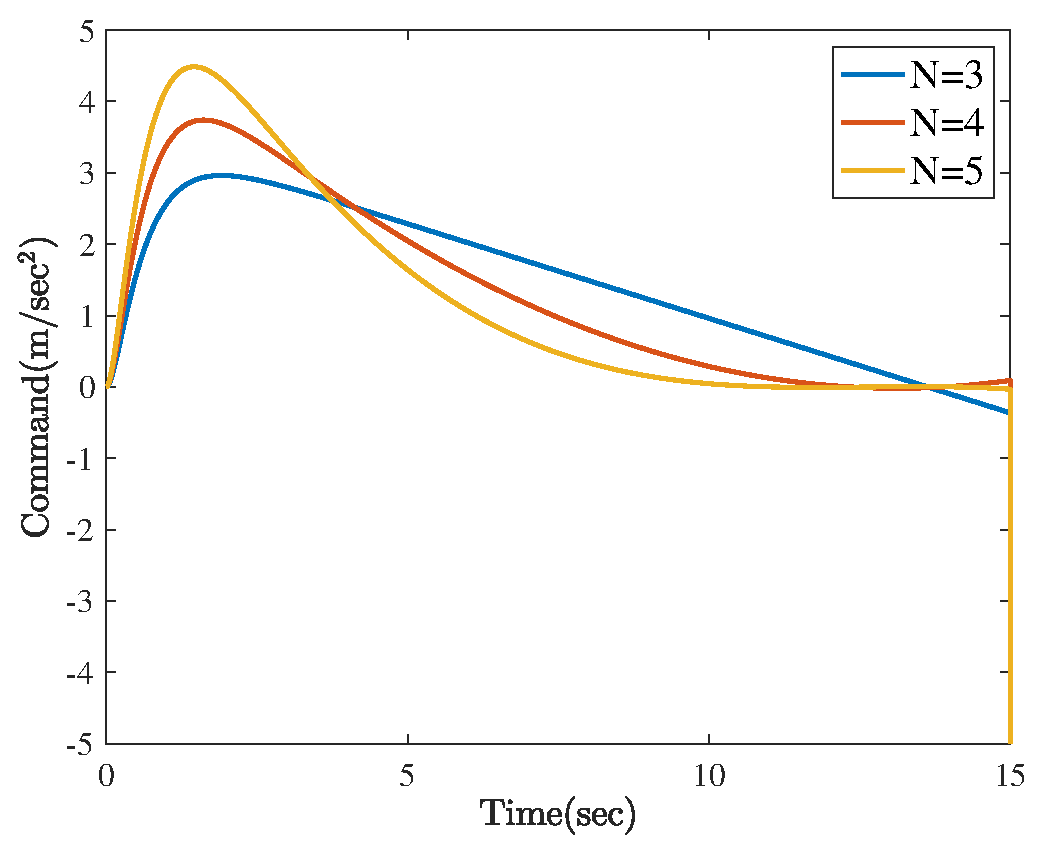
\includegraphics[width=.75\linewidth]{../Figure/Q2/a/command}
\caption{فرمان کنترلی در قانون هدایت تناسبی حقیقی برای ضریب‌های مختلف
$N'$}
\end{figure}

\begin{figure}[H]
	\centering
	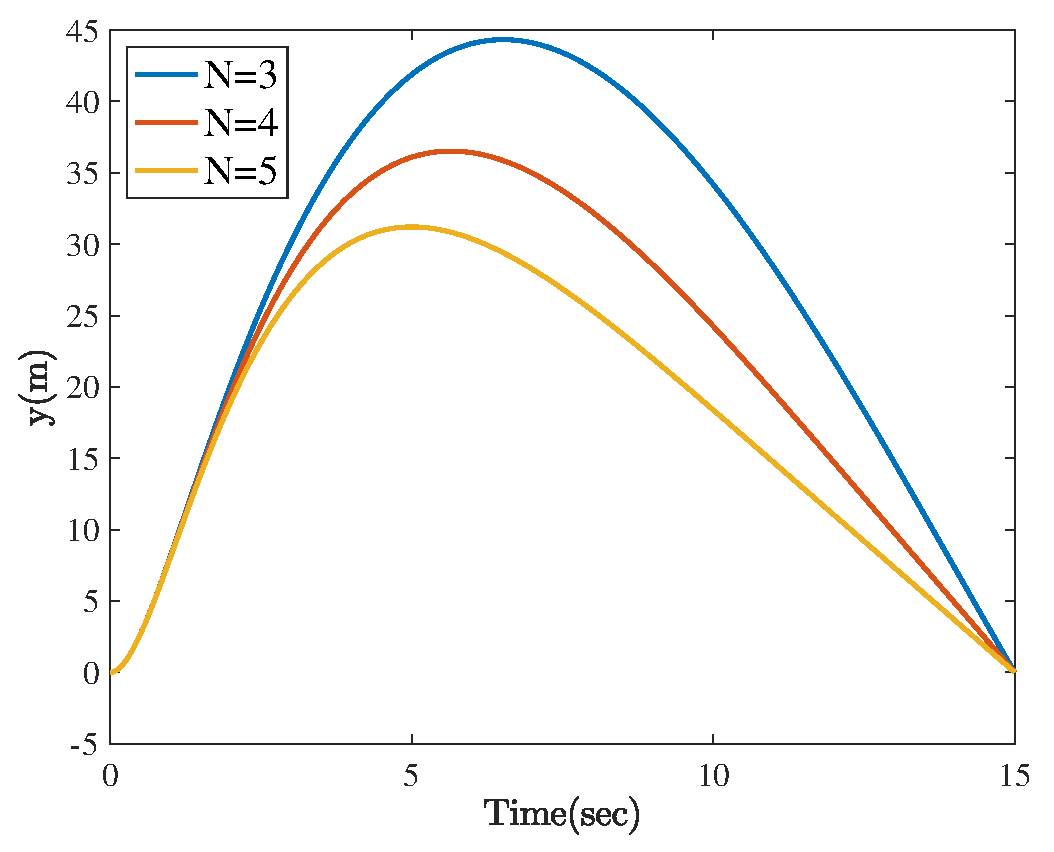
\includegraphics[width=.75\linewidth]{../Figure/Q2/a/y}
	\caption{متغیر \lr{y} در قانون هدایت تناسبی حقیقی برای ضریب‌های مختلف
		$N'$}
\end{figure}
